% ============================================================================
% How the two models connect — the channels of the OG-Core x CLEWS soft link.
% Academic seminar deck: economic interpretation, model representation, and
% validation status. Companion to the methods paper (../paper).
%
% Style: quiet academic formatting (plain titles, minimal colour, no boxes).
% Sources: every frame carries a \note{} with the paper section / repo file it
% draws from. Numbers are the re-blessed golden record; figures under figures/
% are regenerated from the archived coupled battery run (manifest 2026-07-11).
% Merged 2026-08-04 from the prior editorial deck and the channels-explainer
% draft (assertion titles, evidence-layers table, three-capital-channels table).
% Build: latexmk -pdf mechanisms.tex
% ============================================================================
\documentclass[aspectratio=169,11pt]{beamer}

\usepackage[T1]{fontenc}
\usepackage{helvet}
\renewcommand{\familydefault}{\sfdefault}
\usepackage{microtype}
\usepackage{amsmath,amssymb}
\usepackage{graphicx}
\usepackage{booktabs}
\usepackage{tabularx}
\usepackage{array}
\usepackage{tikz}
\usetikzlibrary{arrows.meta,positioning}
\usefonttheme{professionalfonts}

% OG-Core x CLEWS — shared color palette.
% Single source of truth, mirrored from ogclews_link/style.py (the matplotlib figure
% theme) so the TikZ diagrams, the Beamer deck, and the data figures all share one
% editorial, colorblind-safe palette. \input this from any preamble; it only defines
% colors (no package loads), so it is safe in both standalone and beamer documents.

\definecolor{ink}{HTML}{222222}      % primary text / heavy rules
\definecolor{sub}{HTML}{555555}      % secondary text
\definecolor{mute}{HTML}{888888}     % tertiary / source lines
\definecolor{grid}{HTML}{E6E6E6}     % faint rules, fills

% the two models + policy — the load-bearing semantic colors
\definecolor{ogc}{HTML}{0F5499}      % OG-Core      (FT oxford blue)
\definecolor{clews}{HTML}{0D7680}    % CLEWS/OSeMOSYS (teal)
\definecolor{policy}{HTML}{E3120B}   % policy lever (Economist red)

% accents / signed values (match style.py)
\definecolor{claret}{HTML}{990F3D}   % kicker rule
\definecolor{gain}{HTML}{2166AC}     % positive change (blue)
\definecolor{loss}{HTML}{B2182B}     % negative change (red)
\definecolor{amber}{HTML}{E69F00}    % categorical 4
\definecolor{purple}{HTML}{7A6FAC}   % categorical 5
\definecolor{slate}{HTML}{7F8C8D}    % categorical 6 / neutral

% sequential blue ramp (ordered income groups, poorest -> richest)
\definecolor{seqA}{HTML}{C6DBEF}
\definecolor{seqB}{HTML}{9ECAE1}
\definecolor{seqC}{HTML}{6BAED6}
\definecolor{seqD}{HTML}{4292C6}
\definecolor{seqE}{HTML}{2171B5}
\definecolor{seqF}{HTML}{08519C}
\definecolor{seqG}{HTML}{08306B}

\graphicspath{{diagrams/}{figures/}{../results/figures/}}

% ---- quiet academic theme ----------------------------------------------------
\setbeamertemplate{navigation symbols}{}
\setbeamercolor{normal text}{fg=ink,bg=white}
\setbeamercolor{frametitle}{fg=ink,bg=white}
\setbeamercolor{structure}{fg=ink}
\setbeamercolor{itemize item}{fg=sub}
\setbeamercolor{itemize subitem}{fg=sub}
\setbeamerfont{frametitle}{series=\bfseries,size=\large}
\setbeamerfont{title}{series=\bfseries}
\setbeamertemplate{itemize item}{\small\raise0.5pt\hbox{\textbullet}}
\setbeamertemplate{itemize subitem}{\footnotesize\raise0.5pt\hbox{--}}

\setbeamertemplate{frametitle}{%
  \vspace{0.40cm}%
  \usebeamerfont{frametitle}\insertframetitle\par
  \vspace{1.5pt}{\color{grid}\hrule height 0.6pt}\vspace{1pt}}

\setbeamertemplate{footline}{%
  \hbox to\paperwidth{\hspace{0.5cm}%
    {\color{mute}\tiny The channels of the OG-Core--CLEWS link}%
    \hfill{\color{mute}\tiny\insertframenumber\,/\,\inserttotalframenumber}%
    \hspace{0.5cm}}%
  \vspace{3pt}}

% quiet flow boxes: light tint for model identity, thin gray borders
\tikzset{
  sig/.style={draw=black!35, fill=clews!7, rounded corners=1.5pt, inner sep=5pt,
              font=\footnotesize, align=center, text=ink},
  wdg/.style={draw=black!35, fill=ogc!7, rounded corners=1.5pt, inner sep=5pt,
              font=\footnotesize, align=center, text=ink},
  eff/.style={draw=black!35, fill=black!4, rounded corners=1.5pt, inner sep=5pt,
              font=\footnotesize, align=center, text=ink},
  pol/.style={draw=black!35, fill=policy!6, rounded corners=1.5pt, inner sep=5pt,
              font=\footnotesize, align=center, text=ink},
  ch/.style={-{Stealth[length=2mm]}, semithick, draw=sub},
}
\newcommand{\chainrow}[3]{%
  \begin{tikzpicture}[node distance=6mm]
    \node[sig] (a) {#1};
    \node[wdg, right=of a] (b) {#2};
    \node[eff, right=of b] (c) {#3};
    \draw[ch] (a) -- (b); \draw[ch] (b) -- (c);
  \end{tikzpicture}}

% figure frame: title + full-width figure + small gray source line
\newcommand{\figframe}[3]{%
  \begin{frame}{#1}%
    \centering
    \includegraphics[width=\linewidth,height=0.64\textheight,keepaspectratio]{#2}\par
    \vspace{2pt}{\raggedright\color{mute}\scriptsize #3\par}%
  \end{frame}}
\newcommand{\dgmframe}[3]{%
  \begin{frame}{#1}%
    \centering
    \includegraphics[width=\linewidth,height=0.70\textheight,keepaspectratio]{diagrams/#2.pdf}\par
    \vspace{3pt}{\raggedright\color{mute}\scriptsize #3\par}%
  \end{frame}}
\newcommand{\srcnote}[1]{\note{[Sources] #1}}

% ---- notation ------------------------------------------------------------------
\newcommand{\OGCore}{\textsc{OG-Core}}
\newcommand{\CLEWS}{\textsc{CLEWS}}
\newcommand{\OSeMOSYS}{\textsc{OSeMOSYS}}
\newcommand{\tauc}{\tau^{c}}
\newcommand{\taub}{\tau^{b}}
\newcommand{\alphaI}{\alpha_{I}}
\newcommand{\Kg}{K_{g}}
\newcommand{\gammam}{\gamma_{m}}
\newcommand{\rp}{r_{p}}

\title{How the Two Models Connect}
\subtitle{The channels of the OG-Core--CLEWS link:\\
economic interpretation, model representation, and validation status}
\author{Marcelo LaFleur}
\date{August 2026}

\begin{document}

% 1 ----------------------------------------------------------------------------
\begin{frame}[plain]
  \vfill
  {\usebeamerfont{title}\LARGE\color{ink}How the Two Models Connect}\par\vspace{7pt}
  {\large\color{sub}The channels of the OG-Core--CLEWS soft link:\\
   economic interpretation, model representation, and validation status}\par\vspace{18pt}
  {\small\color{mute}Marcelo LaFleur · August 2026 ·
   numbers from the Philippine reference run}\par
  \vfill
  \srcnote{paper/sections/01-introduction.tex; the committed golden record.}
\end{frame}

% 2 ----------------------------------------------------------------------------
\begin{frame}{Neither model alone can say who bears an energy transition}
  \begin{columns}[T,onlytextwidth]
    \begin{column}{0.47\textwidth}
      {\color{clews}\bfseries CLEWS / OSeMOSYS}\par\smallskip
      {\small a least-cost optimiser: chooses what to build and run so energy demand
       is met at the lowest discounted system cost}\par\smallskip
      {\small\begin{itemize}\setlength\itemsep{3pt}
        \item \textbf{rich:} technology, operation, emissions, land \& water
        \item \textbf{blind:} demand is \emph{fixed} --- no price response, no
              households, no government budget, no distribution
      \end{itemize}}
    \end{column}
    \begin{column}{0.47\textwidth}
      {\color{ogc}\bfseries OG-Core}\par\smallskip
      {\small overlapping-generations general equilibrium: households by age $S$
       $\times$ lifetime income $J$, $M$ industries, a government that closes its
       budget each period}\par\smallskip
      {\small\begin{itemize}\setlength\itemsep{3pt}
        \item \textbf{rich:} behaviour, saving, fiscal policy, incidence, demography
        \item \textbf{blind:} no energy technology --- energy is not a priced
              input to production
      \end{itemize}}
    \end{column}
  \end{columns}
  \bigskip
  {\color{sub}\small Each is detailed exactly where the other is blank, so what
  crosses the seam differs by direction: \textbf{quantities} flow from the economy;
  \textbf{prices and physical outcomes} flow from the energy system.}
  \srcnote{paper/sections/03-models.tex; paper/sections/04-framework.tex.}
\end{frame}

% 3 ----------------------------------------------------------------------------
\dgmframe{Quantities flow one way; prices and outcomes flow the other}{architecture}{%
  From the economy: energy demand and the interest rate. From the energy system:
  the energy price, build cost, and emissions. The models stay separate and pass a
  small set of auditable signals --- that asymmetry is the design, not an
  accident.}

% 4 ----------------------------------------------------------------------------
\begin{frame}{Why a staged soft link, not one model}
  \textbf{The classic hard-link route is foreclosed structurally:}
  {\small\begin{itemize}\setlength\itemsep{3pt}
    \item \OGCore{} solves an overlapping-generations \emph{transition path}
          period by period; \OSeMOSYS{} is one perfect-foresight optimisation over
          all years at once
    \item hard links fold the economy in through a scalar welfare objective ---
          and an OLG economy, an equilibrium among cohorts, has none to offer
  \end{itemize}}
  \medskip
  \textbf{So the link runs in stages:}
  \smallskip
  \begin{center}\small
  \resizebox{0.98\linewidth}{!}{%
  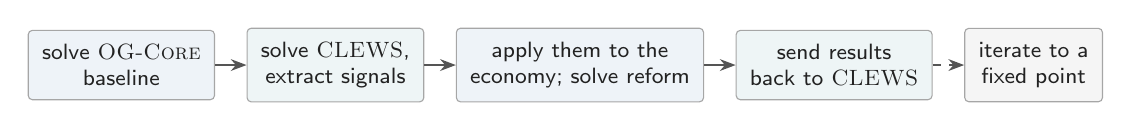
\begin{tikzpicture}[node distance=4mm]
    \node[wdg] (a) {solve \OGCore{}\\baseline};
    \node[sig, right=of a] (b) {solve \CLEWS{},\\extract signals};
    \node[wdg, right=of b] (c) {apply them to the\\economy; solve reform};
    \node[sig, right=of c] (d) {send results\\back to \CLEWS{}};
    \node[eff, right=of d] (e) {iterate to a\\fixed point};
    \draw[ch] (a) -- (b); \draw[ch] (b) -- (c); \draw[ch] (c) -- (d);
    \draw[ch, dashed] (d) -- (e);
  \end{tikzpicture}}
  \end{center}
  \smallskip
  {\color{sub}\small Validated today: the single pass (solid) and the re-solve seam
  the loop requires. The outer iteration (dashed) is designed, not yet wired.}
  \srcnote{paper/sections/04-framework.tex, architecture; ass:hardlink.}
\end{frame}

% 5 ----------------------------------------------------------------------------
\begin{frame}{The deployed price is a levelized-cost proxy, not a marginal price}
  \small The theoretically clean signal is the marginal cost of electricity ---
  what one more unit would cost the least-cost system to supply; under the
  competitive reading, the price that quantity would fetch. In this application it
  is \emph{degenerate}: it binds in scattered years and is near zero elsewhere.
  \smallskip

  \textbf{Four hygiene tests, applied before any marginal cost crosses the seam:}
  {\small\begin{enumerate}\setlength\itemsep{2pt}
    \item above the solver's own reporting resolution;
    \item invariant across alternate optima --- a price that moves while nothing
          physical changes is degeneracy, not information;
    \item decomposed against any cost parameter that floors it;
    \item traceable to a sourced input.
  \end{enumerate}}
  \smallskip
  The electricity signal fails the first two, so the deployed price is the
  \textbf{levelized cost of electricity} --- dense and robust; the Philippine
  reform raises it about $5\%$ on average, reaching $16\%$ by 2030.
  \smallskip

  {\color{sub}\small A fixed point formed with this price is consistency under the
  selected proxy, not a competitive-equilibrium price.}
  \srcnote{paper/sections/04-framework.tex, the LCOE subsection and rem:hygiene;
  paper/sections/06-calibration.tex.}
\end{frame}

% 7a ---------------------------------------------------------------------------
\begin{frame}{Who pays when electricity gets $5\%$ dearer --- and how the model charges them}
  \centering
  \renewcommand{\arraystretch}{1.12}
  {\scriptsize
  \begin{tabularx}{\textwidth}{@{}>{\raggedright\arraybackslash}p{0.20\textwidth} c >{\raggedright\arraybackslash}p{0.21\textwidth} >{\raggedright\arraybackslash}X >{\raggedright\arraybackslash}p{0.20\textwidth}@{}}
    \toprule
    Buyer & Share & In \OGCore{}? & How the channel charges them & What it delivers \\
    \midrule
    \textbf{Industries}\newline (electricity as an input) & $\sim\tfrac34$ &
      \textbf{missing} --- no firm buys from any firm &
      cost-push by hand: $Z_j \mathrel{/}= 1+\varphi_j(g{-}1)$, with $\varphi_j$ =
      each industry's electricity cost share from the SAM &
      the \emph{real resource cost} (contractionary) \\
    \textbf{Households}\newline (electricity bills) & $\sim\tfrac14$ &
      present, via the energy good &
      price wedge $1+\tauc \leftarrow g\,(1+\tauc)$; revenue rebated lump-sum via
      the transfer share $\alpha_T$ &
      \emph{relative price + incidence}, fiscally neutral \\
    \emph{Electricity's self-use} & --- & --- & removed from $\varphi$ &
      each peso enters \emph{once} \\
    \bottomrule
  \end{tabularx}}
  \par\smallskip
  {\raggedright\footnotesize The partition is the design: the wedge is deliberately
  revenue-neutral --- a price rise is a resource cost, not a tax; unrebated, it would
  smuggle in a fiscal consolidation --- and the resource cost is carried on the
  production side, sized by the SAM.\par}
  \srcnote{paper/sections/04-framework.tex, who-pays subsection;
  channels.py energy\_price / energy\_cost\_push; \_recycle\_via\_transfers.}
\end{frame}

% 7b ---------------------------------------------------------------------------
\begin{frame}{Why the firm-side route alone reaches only a quarter of the shock}
  \small Prices in \OGCore{} are outcomes, not dials --- but $p_m\propto 1/Z_m$
  under zero-profit pricing, so lowering electricity's $Z$ makes the model produce
  the higher price \emph{endogenously}. Follow it:
  \medskip

  \centering
  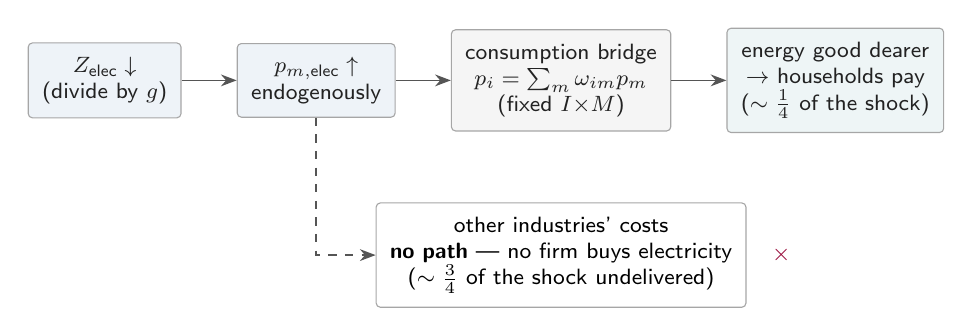
\begin{tikzpicture}[node distance=5mm and 7mm]
    \node[wdg] (z) {$Z_{\text{elec}}\downarrow$\\(divide by $g$)};
    \node[wdg, right=of z] (pm) {$p_{m,\text{elec}}\uparrow$\\endogenously};
    \node[eff, right=of pm] (io) {consumption bridge\\$p_i=\sum_m \omega_{im}p_m$\\(fixed $I{\times}M$)};
    \node[sig, right=of io] (hh) {energy good dearer\\$\to$ households pay\\($\sim\tfrac14$ of the shock)};
    \node[draw=black!35, fill=white, rounded corners=1.5pt, inner sep=5pt,
          font=\footnotesize, align=center, below=9mm of io] (dead)
          {other industries' costs\\\textbf{no path} --- no firm buys electricity\\($\sim\tfrac34$ of the shock undelivered)};
    \draw[ch] (z) -- (pm); \draw[ch] (pm) -- (io); \draw[ch] (io) -- (hh);
    \draw[ch, dashed] (pm.south) |- (dead.west);
    \node[font=\footnotesize\bfseries, text=claret, right=2mm of dead.east] {$\times$};
  \end{tikzpicture}
  \medskip

  {\raggedright\footnotesize The route is correct but \emph{incomplete by
  construction}: the only electricity buyers in the model are households --- and it
  encodes a system-cost change as an electricity-technology change. Hence the split:
  the wedge for the household quarter, the SAM-sized cost-push for the industrial
  three quarters, until firms buy electricity inside the model.\par}
  \srcnote{channels.py energy\_price\_tfp docstring; ogcore firm.py get\_pm,
  SS.py:277 (p\_i = io\_matrix @ p\_m).}
\end{frame}

% 8 ----------------------------------------------------------------------------
\begin{frame}{The eight channels}
  \centering\scriptsize
  \renewcommand{\arraystretch}{1.05}
  \begin{tabularx}{\textwidth}{@{}>{\bfseries}p{0.18\textwidth} c >{\raggedright\arraybackslash}p{0.26\textwidth} >{\raggedright\arraybackslash}X@{}}
    \toprule
    Channel & Dir. & Quantity entering the interface & Model representation \\
    \midrule
    Energy price & C$\to$O & reform/baseline cost ratio & industry cost-push + household wedge \\
    Public investment & C$\to$O & grid \& transmission build cost & $\alphaI \to \Kg$ \\
    Capital intensity & C$\to$O & fleet capital-cost share & energy industry's capital share $\gammam$ \\
    Health & C$\to$O & PM$_{2.5}$ emissions path & survival rates + effective labour \\
    Carbon price & policy & exogenous price path & emissions penalty (energy side) + optional household wedge \\
    Investment incentive & policy & tax-credit rate & user cost of capital \\
    Discount rate & O$\to$C & equilibrium return & planning-rate input \\
    Energy demand & O$\to$C & activity ($Y_m$ or $C_i$) & annual demand path \\
    \bottomrule
  \end{tabularx}
  \par\medskip
  {\color{sub}\small The point: nothing crosses the boundary informally. Every
  exchanged quantity is one of these eight named, guarded channels --- four in,
  two policy, two back.}
  \srcnote{paper/sections/05-channels.tex, Table 1; ogclews\_link/channels.py.}
\end{frame}

% 9 ----------------------------------------------------------------------------
\begin{frame}{Carbon costs enter once}
  \begin{columns}[T,onlytextwidth]
    \begin{column}{0.47\textwidth}
      {\bfseries Design}\par\smallskip
      {\small\begin{itemize}\setlength\itemsep{3pt}
        \item energy side: an emissions penalty changes technology costs and the
              optimal build
        \item economy side: a household wedge can price direct carbon content,
              with revenue recycled
        \item one price, once --- never also read back from the energy model's
              own implied carbon cost
      \end{itemize}}
    \end{column}
    \begin{column}{0.47\textwidth}
      {\bfseries In the application (verified)}\par\smallskip
      {\small The Philippine reform solve carries \emph{no} emissions penalty ---
      it is a policy-composition scenario --- so \textbf{no carbon price acts in
      the reported coupled numbers}. The flagship run \emph{emits} a
      \$50/tCO$_2$ input for the energy model's next solve; the $-0.021\%$
      standalone result is the household-wedge experiment run by itself.}
    \end{column}
  \end{columns}
  \medskip
  {\color{sub}\small Provenance checked in the case's own compiled solver input:
  \texttt{EmissionsPenalty} is empty in both the baseline and reform runs.}
  \srcnote{paper/sections/05-channels.tex, carbon; the round-2 provenance check in
  docs/design/methods-paper-review-follow-up-response.md (data.txt, Base\_v9 and
  PEP\_v9).}
\end{frame}

% 10 ---------------------------------------------------------------------------
\begin{frame}{Three capital mechanisms act on different equations}
  \footnotesize
  \renewcommand{\arraystretch}{1.12}
  \begin{tabularx}{\textwidth}{@{}>{\bfseries}p{0.19\textwidth} >{\raggedright\arraybackslash}p{0.22\textwidth} >{\raggedright\arraybackslash}p{0.20\textwidth} >{\raggedright\arraybackslash}X@{}}
    \toprule
    Mechanism & Economic object & Model entry & Interpretation \\
    \midrule
    Public investment & grid and transmission & $\alphaI \to \Kg$ & productive public capital; debt financing can crowd out private investment \\
    Capital intensity & production factor mix & energy-industry $\gammam$ & changes factor shares, unit cost, and the electricity price \\
    Investment incentive & private capital incentive & tax credit in the user cost & shifts private capital demand toward generation \\
    \bottomrule
  \end{tabularx}
  \bigskip
  {\small The capital-share lever and the investment incentive are \emph{not}
  interchangeable views of one build-out: they act on different equations, can move
  energy capital in opposite directions, and the accounting discipline forbids
  stacking them. Public and private capital are distinct objects --- coupling both
  is complementary, not double counting.}
  \srcnote{paper/sections/05-channels.tex, the capital pair;
  paper/sections/04-framework.tex, principles.}
\end{frame}

% 11 ---------------------------------------------------------------------------
\begin{frame}{Raising the capital share sheds capital; the tax credit draws it in}
  \small
  The first-order condition: capital is held in proportion to \emph{revenue},
  \(K_E=\gamma_E\,p_E Y_E/\rho_E\) (share $\times$ revenue $\div$ cost of
  capital). What the lever actually does:
  \smallskip

  \centering
  \renewcommand{\arraystretch}{1.05}
  {\footnotesize
  \begin{tabular}{@{}clr@{}}
    \toprule
    & What happens & Measured \\
    \midrule
    1 & the lever raises the capital exponent & $\gamma_E$ $+12.2\%$ \\
    2 & production gets cheaper; zero profit passes the cut into the price & $p_E$ $-42.8\%$ \\
    3 & cheaper electricity raises demand and output & $Y_E$ $+20.9\%$ \\
    4 & revenue $p_E Y_E$ \emph{falls} --- the price collapse outweighs the output gain & \\
    5 & capital is a share of revenue, so capital \emph{falls} & $K_E$ $-22.4\%$ \\
    \bottomrule
  \end{tabular}}
  \par\smallskip
  {\raggedright\footnotesize The identity $\hat K_E=\hat\gamma_E\,\hat p_E\,\hat Y_E$
  reproduces the $-22.4\%$ to within $0.023$\,pp: the attribution is exact, not a
  narrative.\par}
  \smallskip

  {\raggedright\textbf{The conclusion, stated plainly:} a higher capital
  \emph{share} is not capital attraction. The instrument that attracts capital is
  the investment tax credit --- it lowers the cost of capital $\rho_E$ in the
  denominator, where $\gamma_E$ does not appear. Two levers, two different
  equations, opposite effects on energy capital: never stack them.\par}
  \smallskip
  {\raggedright\color{sub}\scriptsize Evidence: recomputed from the archived M=8
  solved steady states (2026-08-04); a re-run under the re-blessed baseline is
  queued.\par}
  \srcnote{paper/sections/05-channels.tex, Table 2; SS\_vars recompute in
  docs/design/methods-paper-review-response.md.}
\end{frame}

% 12 ---------------------------------------------------------------------------
\begin{frame}{Cleaner air pays through workers now, and adds retirees later}
  \begin{columns}[T,onlytextwidth]
    \begin{column}{0.50\textwidth}
      {\footnotesize\begin{itemize}\setlength\itemsep{2pt}
        \item \CLEWS{} supplies the PM$_{2.5}$ path; the GBD supplies the burden
              and its age profiles (right)
        \item a calibrated dose-response scales the $2.7\%$ emissions cut to
              $\sim$95 fewer deaths/year (not the $1{,}165$ of one-for-one scaling)
        \item \textbf{mortality} skews elderly $\to$ saved lives add retirees
              $\to$ long-run output $\approx 0$
        \item \textbf{morbidity} is working-age $\to$ effective labour rises
              ($+0.19\%$ near-term)
      \end{itemize}}
      \smallskip
      {\footnotesize\textbf{So the GDP effect changes sign with the horizon} ---
      gain on the path, cost in the steady state; only an age-structured model
      produces that split. (The morbidity elasticity is an application
      assumption.)}
    \end{column}
    \begin{column}{0.46\textwidth}
      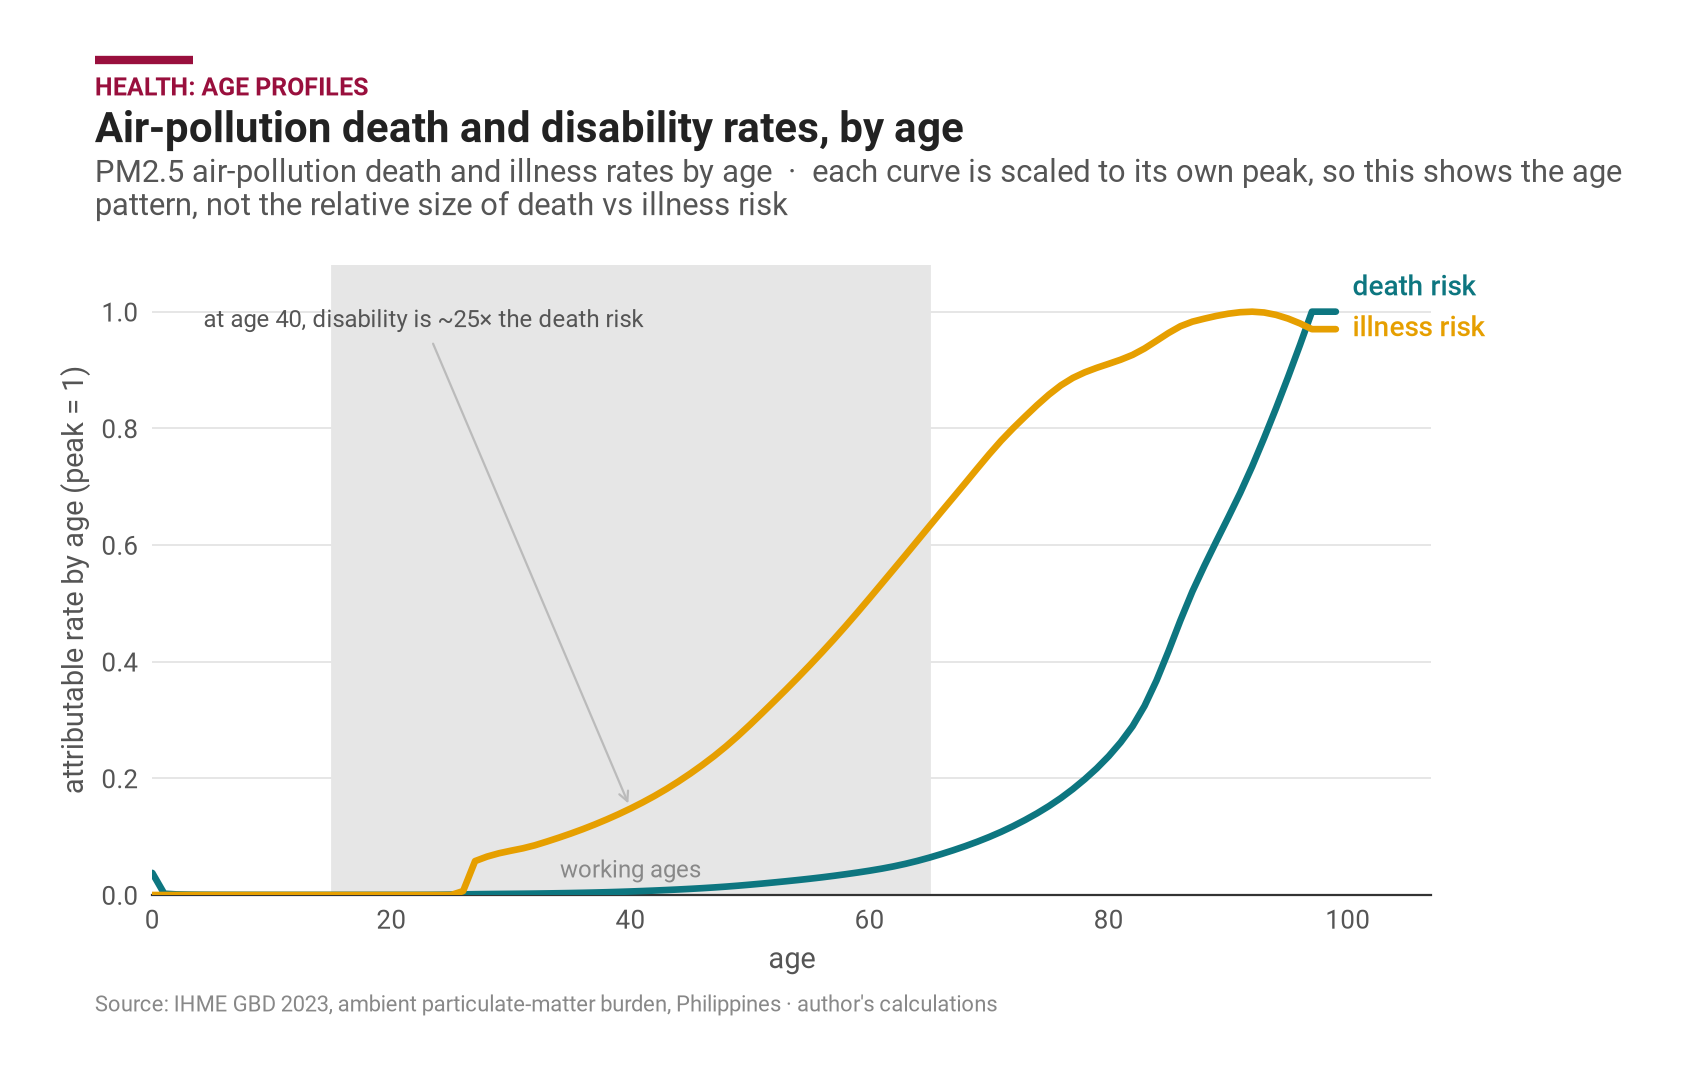
\includegraphics[width=\linewidth,height=0.60\textheight,keepaspectratio]{health_age_profiles.png}
    \end{column}
  \end{columns}
  \srcnote{paper/sections/05-channels.tex, health; figures regenerated from the
  archived coupled run; ogclews\_link/data/pm25\_health.json.}
\end{frame}

% 13 ---------------------------------------------------------------------------
\begin{frame}{The economy answers back: its return and its demand}
  \begin{columns}[T,onlytextwidth]
    \begin{column}{0.47\textwidth}
      {\bfseries Discount rate}\par\smallskip
      {\small The equilibrium return $\rp$ becomes the energy system's planning
      rate --- a harmonisation convention, not a structural equality.}\par\smallskip
      {\small\emph{Still to establish:}
      \begin{itemize}\setlength\itemsep{2pt}
        \item social rate vs financing cost
        \item real/nominal and annualisation conventions
        \item risk and tax adjustments
      \end{itemize}}
    \end{column}
    \begin{column}{0.47\textwidth}
      {\bfseries Energy demand}\par\smallskip
      {\small Sectoral output or consumption scales annual energy-service
      demand.}\par\smallskip
      {\small\emph{Current evidence:}
      \begin{itemize}\setlength\itemsep{2pt}
        \item the artifact is produced after the economy solves
        \item a controlled $+10\%$ demand patch re-solves the energy model and
              raises production $+4.3\%$
        \item the emitted artifact has not yet passed end to end --- that is the
              outer controller's job
      \end{itemize}}
    \end{column}
  \end{columns}
  \medskip
  {\color{sub}\small Both are inert in a single pass by construction; they move the
  economy only once the loop iterates.}
  \srcnote{paper/sections/05-channels.tex, discount rate and demand;
  docs/design/INTEGRATION-HANDOFF.md (the +10\% seam test).}
\end{frame}

% 14 ---------------------------------------------------------------------------
\dgmframe{Closing the loop}{loop}{%
  Iterate until energy demand stops changing. The re-solve seam is built and tested
  (a controlled $+10\%$ demand patch moved production $+4.3\%$); what remains is the
  outer iteration and its damping.}

% 15 ---------------------------------------------------------------------------
\begin{frame}{Counting each cost once: five principles}
  \small
  \begin{enumerate}\setlength\itemsep{4pt}
    \item \textbf{One carbon price} --- an energy-side penalty and an economy-side
          wedge on the same path; never also inferred from the energy model's
          implied carbon cost.
    \item \textbf{Count each energy cost once} --- the energy channel partitions
          electricity by use, self-use netted; a second representation of the same
          flow is forbidden.
    \item \textbf{One view of generation capital} --- cost-push \emph{or} an
          investment credit; the capital share is not a third interchangeable view.
    \item \textbf{Revenue must be routed} --- recycle or finance the mechanical
          wedge revenue, or a hidden fiscal expansion rides along.
    \item \textbf{Public and private capital are distinct} --- $\alphaI\to\Kg$ and
          the firm's own $K$ touch different objects.
  \end{enumerate}
  \medskip
  {\color{sub}\small Enforced by guards in the code where a forbidden combination
  can arise within a channel, and by experiment-composition rules across channels.}
  \srcnote{paper/sections/04-framework.tex, principles (enforcement wording after
  the 2026-08-04 review round).}
\end{frame}

% 16 ---------------------------------------------------------------------------
\begin{frame}{Three mechanisms drive the Philippine results: price, investment, health}
  \centering
  \resizebox{0.98\textwidth}{!}{%
  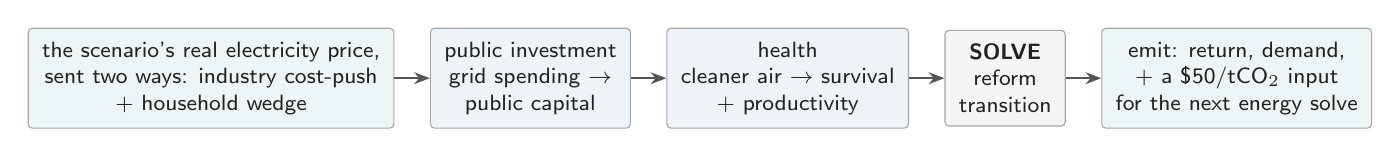
\begin{tikzpicture}[node distance=4.5mm and 4.5mm]
    \node[sig] (a) {the scenario's real electricity price,\\sent two ways: industry cost-push\\$+$ household wedge};
    \node[wdg, right=of a] (b) {public investment\\grid spending $\to$\\public capital};
    \node[wdg, right=of b] (d) {health\\cleaner air $\to$ survival\\$+$ productivity};
    \node[eff, right=of d] (s) {\textbf{SOLVE}\\reform\\transition};
    \node[sig, right=of s] (f) {emit: return, demand,\\$+$ a \$50/tCO$_2$ input\\for the next energy solve};
    \draw[ch] (a) -- (b); \draw[ch] (b) -- (d);
    \draw[ch] (d) -- (s); \draw[ch] (s) -- (f);
  \end{tikzpicture}}
  \medskip
  \begin{columns}[T,onlytextwidth]
    \begin{column}{0.52\textwidth}
      {\footnotesize\begin{itemize}\setlength\itemsep{4pt}
        \item three mechanisms act: price, investment, health; the emitted signals
              are inert in one pass (no carbon price acts here)
        \item the steady-state total is not the sum of the standalone runs ---
              they do not duplicate this treatment
        \item incidence is regressive under full recycling
              ($C_{ss}=-0.092\%$ in the recycled experiment)
      \end{itemize}}
    \end{column}
    \begin{column}{0.42\textwidth}
      \renewcommand{\arraystretch}{1.1}
      {\scriptsize
      \begin{tabular}{@{}lrrr@{}}
      \toprule
      \% vs baseline & steady & $t_0$ & $t_{10}$ \\
      \midrule
      output $Y$ & $-0.138$ & $+0.179$ & $+0.202$ \\
      consumption $C$ & $-0.087$ & $+0.066$ & $+0.385$ \\
      \bottomrule
      \end{tabular}}
    \end{column}
  \end{columns}
  \srcnote{paper/sections/07-results.tex; ogclews\_link/experiments.py, coupled;
  results/golden.json.}
\end{frame}

% 17 ---------------------------------------------------------------------------
\figframe{Each mechanism alone moves output little}{golden_channel_impact}{%
  Standalone mechanism experiments, steady-state output impact (the figure's ``by
  channel'' title predates the channel/experiment distinction). The energy price is
  $\approx 0$ honestly transmitted; carbon ($-0.021\%$, the household-wedge
  experiment) is the largest standalone contraction. Source: the committed golden
  record.}

% 18 ---------------------------------------------------------------------------
\figframe{The coupled economy: gains along the path, costs in the long run}{macro_transition}{%
  The coupled transition (\% vs baseline): output $+0.179\%$ near-term, peaking
  about $+0.4\%$ in the early 2040s, then settling toward the $-0.138\%$ steady
  state as the survival gain adds retirees and energy costs persist. The horizon
  split is the health channel's signature and is invisible to a static model.
  Figure regenerated from the archived coupled run.}

% 19 ---------------------------------------------------------------------------
\figframe{Who bears it: lifetime welfare by cohort}{welfare_cev_by_age}{%
  Remaining-lifetime welfare effect by age at the reform, with the income-group
  range. Younger cohorts gain (they live through the healthier transition); cohorts
  near and past retirement bear the cost. This cohort resolution is what the
  overlapping-generations side adds --- no representative-agent partner can produce
  it. Figure regenerated from the archived coupled run.}

% 20 ---------------------------------------------------------------------------
\begin{frame}{Validation is layered, and each layer has a boundary}
  \centering\scriptsize
  \renewcommand{\arraystretch}{1.08}
  \begin{tabularx}{\textwidth}{@{}>{\bfseries}p{0.17\textwidth} >{\raggedright\arraybackslash}X >{\raggedright\arraybackslash}p{0.28\textwidth}@{}}
    \toprule
    Evidence layer & What it establishes & Current boundary \\
    \midrule
    Transform tests & shapes, bounds, concordance, fail-fast behaviour & not an economic calibration \\
    Controlled runs & solve completion, direction, identity checks & some coefficients remain provisional \\
    Golden record & macro aggregates stable against a committed record & excludes emitted artifacts and sectoral detail \\
    Re-solve seam & a demand patch survives case copy, solve, read-back & no emitted artifact passed end to end \\
    Closed-loop test & convergence and error propagation & outer controller not implemented \\
    \bottomrule
  \end{tabularx}
  \bigskip
  {\color{sub}\small ``Validated'' never carries all five meanings at once; each
  claim in the paper is scoped to its layer.}
  \srcnote{paper/sections/07-results.tex, validation; the review conversation in
  docs/design/ (2026-08-04).}
\end{frame}

% 21 ---------------------------------------------------------------------------
\begin{frame}{Where the coupling stands}
  \begin{columns}[T,onlytextwidth]
    \begin{column}{0.47\textwidth}
      {\bfseries Established}\par\smallskip
      {\small\begin{itemize}\setlength\itemsep{3pt}
        \item the full energy-to-economy pass on real inputs: the scenario's real
              electricity price, the real Global Burden of Disease data
        \item controlled validation evidence for the price, capital, and health
              mechanisms
        \item the re-solve seam responds correctly to a controlled demand patch
        \item carbon provenance in the application verified, and the reporting
              corrected to match
      \end{itemize}}
    \end{column}
    \begin{column}{0.47\textwidth}
      {\bfseries Next, in order}\par\smallskip
      {\small\begin{itemize}\setlength\itemsep{3pt}
        \item the matched cumulative decomposition that reproduces the coupled run
        \item regression tests for the emitted artifacts
        \item the capital re-run under the re-blessed baseline
        \item the damped outer controller --- loop closure
        \item the unit bridge, before any submission
      \end{itemize}}
    \end{column}
  \end{columns}
  \bigskip
  {\color{sub}\small One line: a small, auditable library of economic mechanisms ---
  each signal counted once, each claim scoped to its evidence.}
  \srcnote{paper/sections/01-introduction.tex, the frontier paragraph;
  docs/design/methods-paper-review-follow-up-response.md, the queue.}
\end{frame}

\end{document}
